\section{Behaviour}
\label{Behaviour}
\subsection{Field Player Strategy}
The overall strategy for this year was to attempt to kick the ball towards the attacking goal as quickly and as often as possible. To do this the general behaviour was to walk to the kicking position where the attacking goal was lined up and then kick. Since we only kicked forward this was a calculated position based on the position of the ball on the field. In terms of team behaviour, we attempted to always have one robot chasing the ball while any other robots tried to move into their ideal position. In an attempt to simplify the writing of behaviour code the walk engine included many planning functions so that behaviours simply pass the walk engine the desired relative position and heading and the walk engine will take it there. These path planning paths were built around the desired behaviours so many complex decisions were not required. For example when approaching the ball from the front, and therefore a large heading change is required, to prevent the robot walking through the ball on its way to the kicking position a path containing an arc walk is used to move behind the ball and correct the heading. To carry out our overall strategy a number of sub-behaviours were developed. These were run depending on the robots current circumstances as shown in ~\autoref{fig:PlayerTaskDecision}.

\begin{figure}[htpb]
\begin{center}
   \leavevmode
    \scalebox{0.8} {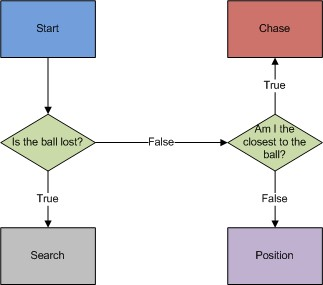
\includegraphics{figs/FieldPlayerTaskDecision.jpg} }
    \caption{Player task decision tree}
    \label{fig:PlayerTaskDecision}
\end{center}
\end{figure}



\subsubsection{Searching}
The trigger for searching was greatly improved upon from last year. Previously the robot would search if it could simply not see the ball. However when moving into position we found that it may be advantageous to lose sight of the ball for short amounts of time to gain an increase in walking speed. Because of this some high level properties were created \emph{isBallLost} and \emph{amILost}. The \emph{isBallLost} property takes into account the number of vision frames since the ball was last seen as well as the current world model uncertainty to determine if yourself or the team as a whole has lost the ball. Because the world model ball also includes information from team mates if they are providing the robot with good estimates of the ball position it may not be required to search. Likewise if the world model uncertainties indicate that the predictions are accurate searching again may not be required. The \emph{amILost} property was used to determine the validity of the robots field location estimates. Once the uncertainty reached a predefined threshold the robot would attempt to localise by doing a pan at a level likely to see the goal posts and field lines.

Once we had determined that a ball was lost and must be found we used a simple searching method. The robot would pan its head vertically from top to bottom while turning in a circle. The horizontal angle of the camera was set to one step worth of a turn towards the turning direction so that if a ball is seen at the completion of the next turn step it can begin moving forwards towards it. We would alternate cameras for each turn starting with the camera we deemed most likely to see the ball based on its estimated distance. However this sometimes proved frustrating since it would sometimes choose the wrong camera and would then require more than a complete turn to find the ball.


\subsubsection{Chasing}
The chasing behaviour is the main part of our game play. It involves walking to an ideal kicking position. turning to line up the goal, then lining up the ball and finally kicking. To simplify the writing of behaviours we created another high level property \emph{isOpponentsGoalLinedUp}. This is determined very simply, if the left hand post of the attacking goal is on our left and the right hand post is on our right then the goal is lined up for a kick. There were a number of states in the chasing behaviour. The transition conditions between states can be found in \autoref{fig:ChasingStateDiagram}.
\begin{enumerate}
\item \textbf{Approach} The robot will move towards the desired kicking position. This is situated on the opposite side of the ball to the attacking goal.
\item \textbf{Position} The robot will turn to face the attacking goal, lining it up so that it is facing between the two posts.
\item \textbf{Kick} The robot will line one of its feet up to the ball. One the ball is within the effective kicking range the kick sequence will be called.
\end{enumerate}

\begin{figure}[htpb]
\begin{center}
   \leavevmode
    \scalebox{0.8} {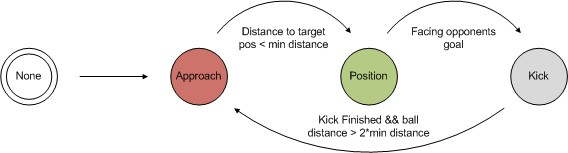
\includegraphics{figs/FieldPlayerChasingStates.jpg} }
    \caption{Chasing behaviour state diagram}
    \label{fig:ChasingStateDiagram}
\end{center}
\end{figure}

\subsubsection{Positioning}
The positioning behaviour simply moves to a fixed point on the field. Once close to the desired field position the robot turns to face the ball. If the ball can be seen the robot will track the ball. If not the robot will face towards the estimated ball position and pan to look for the ball and view localisation landmarks.

\subsection{Goal Keeper Strategy}
The overall goal keeper strategy was to keep the ball from entering the defending goal. This would ideally be achieved by using the goal keeper as an obstacle in the direct path between the ball and the defending goal. If the ball was far away, the goal keeper would spend most of its time searching (same as field player) and positioning between the ball and the defending goal. However, if the ball was close to the goalkeeper, the goal keeper would have to react by either clearing the ball (lining up for a kick towards the attacking goal) or if the ball was moving towards the goal keeper, it would perform a dive to stop the ball from entering the goal. The following subsections will describe in detail the positioning and reactions to the ball. The goal keeper has a higher priority in the over all team behaviour hierarchy. The reasoning behind this is that around the defending goal area, the ball can easily move into an area off limits to a field player, and in this situation the defending the goal is the teams main priority. A decision tree of the goal keeper can be see in ~\autoref{fig:GoalKeeperDecision}.

\begin{figure}[htpb]
\begin{center}
   \leavevmode
    \scalebox{0.8} {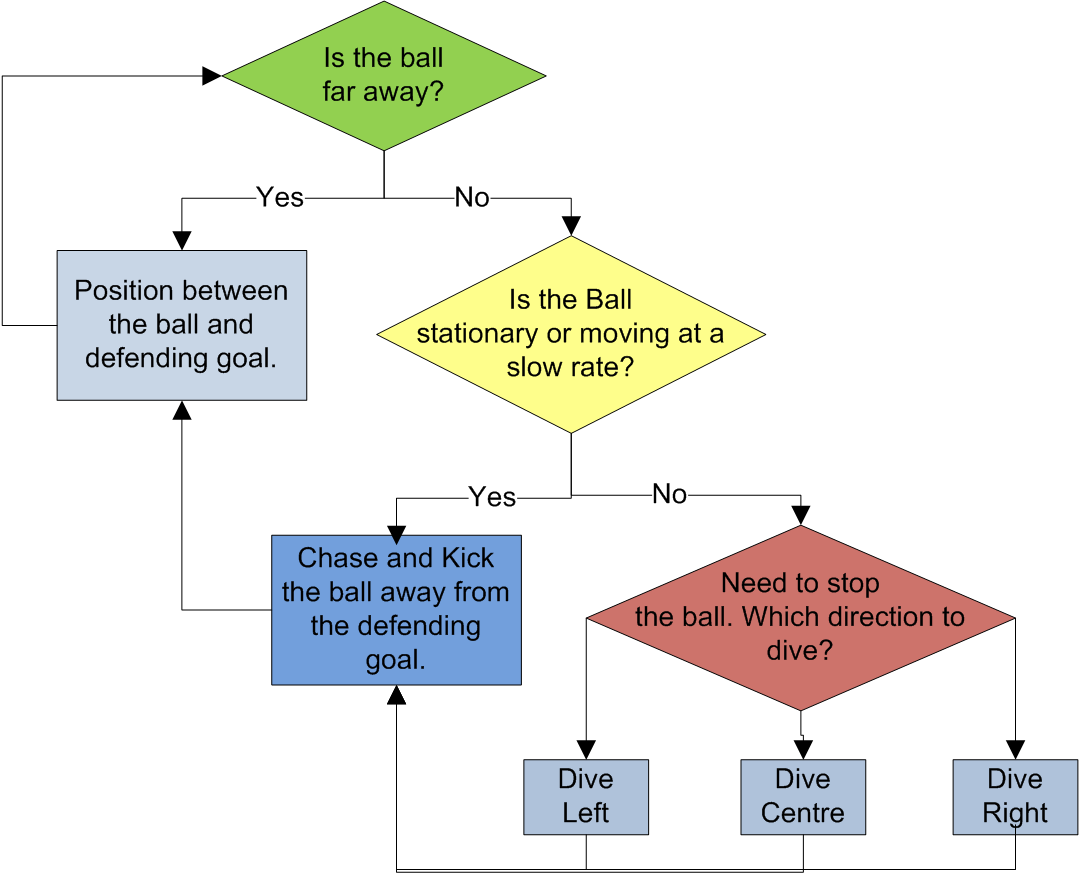
\includegraphics{aaronfigs/GoalKeeperDecisions.png} }
    \caption{Goal Keeper task decision tree}
    \label{fig:GoalKeeperDecision}
\end{center}
\end{figure}

\subsubsection{Positioning}
Unlike other teams in the competition who would simply position their goal keeper in the middle of the goals, we chose to use a more active and aggressive keeper. The positioning module was significantly different to the field player, as the goal keeper is required to attempt to position between the ball and the defending goals at all times. It heavily depended on the localisation information and current position of the ball. Using this information we calculate a position on the field to guard that maximises the coverage of the goal. This was achieved by calculating the ideal path from the ball to the centre of the goals and intersecting this ideal ball path with a boundary, where the boundary is the edge of an area for which we would like the goal keeper to roam with-in.


\subsubsection{Reactions to the Ball}
Once the ball is at a close distance, the goal keeper will react in one of two ways. 

The first is to chase and remove the ball from its defending area in the direction of the attacking goal in a similar manner as the field player. This is only triggered if the ball is stationary or moving very slowly.

The second is a dive which is triggered by a moving ball. When a dive is triggered, the goal keeper will select the best dive from three pre-written dive scripts. There are three dive scripts, Left, Forward and Right. The goal keepers dive selection criteria includes, projecting the ball to intersect its' vertical plane, then selecting the dive that closely corresponds to the intersection. The dive is executed before the ball intersects the goal keeper, so it is able to dive into position to block the balls path. The dive is within required regulation, as it only stays in its dived position for a few seconds before getting up. After the dive it will proceed to chasing and kicking the ball out of the goal area.
